\documentclass[aspectratio=169,11pt]{beamer}
\usetheme{metropolis}
\usepackage{tikz}
\usetikzlibrary{arrows.meta,positioning,decorations.pathmorphing,calc,shapes.geometric}
\usepackage{booktabs}
\usepackage{xcolor}
\usepackage{amsmath}
\usepackage{graphicx}
\usepackage{hyperref}
\hypersetup{colorlinks=true,linkcolor=.,urlcolor=camera,citecolor=camera}
\graphicspath{{../figures/}}

% === Color palette ===
\definecolor{engine}{HTML}{E74C3C}
\definecolor{camera}{HTML}{3498DB}
\definecolor{proof}{HTML}{9B59B6}
\definecolor{counter}{HTML}{E67E22}
\definecolor{neutral}{HTML}{95A5A6}
\definecolor{pass}{HTML}{27AE60}
\definecolor{fail}{HTML}{E74C3C}
\definecolor{sae}{HTML}{E91E63}
\definecolor{causal}{HTML}{2196F3}
\definecolor{circuits}{HTML}{FF9800}
\definecolor{bg}{HTML}{FAFAFA}

\title{Benchmarks Are Engines, Not Cameras}
\subtitle{How ML evaluation tools reshape the knowledge they measure}
\author{Elliot Tower}
\date{2026}
\institute{}

\begin{document}

\maketitle

%% --- SLIDE: Overview ---
\begin{frame}{Overview}
\begin{columns}[T]
\begin{column}{0.48\textwidth}
\textbf{Part 1: The engine metaphor}\\[0.15em]
{\footnotesize%
\quad 1.~The Black-Scholes story\\%
\quad 2.~Camera vs.\ engine\\%
\quad 3.~Performativity and counterperformativity\\%
\quad 4.~Benchmarks do the same thing\\%
\quad 5.~The benchmark lifecycle%
}\vspace{0.6em}

\textbf{Part 2: Proof cultures}\\[0.15em]
{\footnotesize%
\quad 6.~What is mechanistic interpretability?\\%
\quad 7.~Three communities, three standards\\%
\quad 8.~The denominator problem\\%
\quad 9.~Multiple comparisons and FWER%
}
\end{column}
\begin{column}{0.48\textwidth}
\textbf{Part 3: Peer review makes it worse}\\[0.15em]
{\footnotesize%
\quad 10.~The counterperformative loop\\%
\quad 11.~11,196 ICLR submissions\\%
\quad 12.~Simpson's paradox explained\\%
\quad 13.~Simpson's paradox in our data%
}

\vspace{1.8em}
\textbf{Part 4: What to do}\\[0.15em]
{\footnotesize
\quad 14.~Structural interventions\\
\quad 15.~Project limitations\\
\quad 16.~Conclusion
}
\end{column}
\end{columns}
\end{frame}


%% ============================================================
%% PART 1: THE ENGINE METAPHOR
%% ============================================================

\begin{frame}[plain]
\vfill
\begin{center}
  \setlength{\fboxrule}{2.5pt}%
  \fcolorbox{black}{white}{\parbox{0.65\textwidth}{\centering\vspace{0.8em}
    {\Large\bfseries Part 1}\\[0.5em]
    {\large Benchmarks are engines, not cameras}
  \vspace{0.8em}}}
\end{center}
\vfill
\end{frame}

%% --- SLIDE: What is Black-Scholes? ---
\begin{frame}{The Black-Scholes story}

In 1973, Fischer Black and Myron Scholes published a formula for pricing options --- the \href{https://en.wikipedia.org/wiki/Black\%E2\%80\%93Scholes_model}{Black-Scholes model}.

\vspace{0.5em}

Before it, options pricing was mostly intuition and guesswork. Different traders quoted wildly different prices for the same contract.

\vspace{0.5em}

The formula said: given a stock price, volatility, time to expiry, and interest rate, there is \textbf{one correct price} for every option.

\vspace{0.8em}

\begin{center}

\begin{tikzpicture}
  \draw[neutral,thick,rounded corners,fill=neutral!5] (0,0) rectangle (10,1.2);
  \node[font=\small,align=center] at (5,0.6) {$C = S\,\Phi(d_1) - K\,e^{-rT}\Phi(d_2)$};
\end{tikzpicture}
\end{center}

\vspace{0.3em}
{\small The same year, the \href{https://en.wikipedia.org/wiki/Chicago_Board_Options_Exchange}{Chicago Board Options Exchange} opened. Traders carried printouts of Black-Scholes pricing tables onto the trading floor.}
\end{frame}

%% --- SLIDE: What happened next ---
\begin{frame}{The model made itself true}

At first, actual option prices \textbf{deviated} from Black-Scholes predictions.

\vspace{0.5em}

Then something strange happened. Over the next decade, market prices \textbf{converged} toward the formula's predictions.

\vspace{0.8em}

\begin{center}
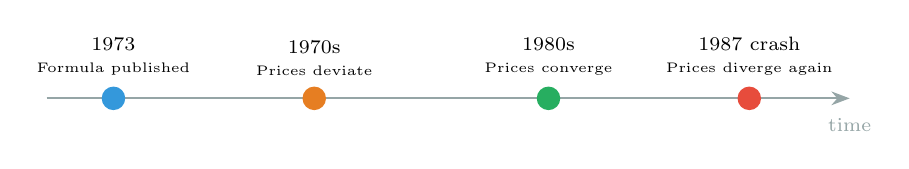
\begin{tikzpicture}[scale=0.85]
  % Timeline
  \draw[neutral,thick,-{Stealth}] (0,0) -- (12,0);
  \node[font=\scriptsize,neutral] at (12,-0.4) {time};

  % 1973
  \fill[camera] (1,0) circle (5pt);
  \node[font=\scriptsize,align=center,above] at (1,0.2) {1973\\{\tiny Formula published}};

  % Early: deviation
  \fill[counter] (4,0) circle (5pt);
  \node[font=\scriptsize,align=center,above] at (4,0.2) {1970s\\{\tiny Prices deviate}};

  % Convergence
  \fill[pass] (7.5,0) circle (5pt);
  \node[font=\scriptsize,align=center,above] at (7.5,0.2) {1980s\\{\tiny Prices converge}};

  % 1987
  \fill[engine] (10.5,0) circle (5pt);
  \node[font=\scriptsize,align=center,above] at (10.5,0.2) {1987 crash\\{\tiny Prices diverge again}};
\end{tikzpicture}
\end{center}

\vspace{0.5em}

The formula didn't \emph{describe} a pre-existing reality. Traders using the formula \textbf{created the reality it described}. And when the assumptions broke in 1987, prices diverged just as fast.
\end{frame}

%% --- SLIDE: Camera vs engine ---
\begin{frame}{Camera vs.\ engine}

The sociologist Donald MacKenzie studied this episode in \href{https://mitpress.mit.edu/9780262134606/an-engine-not-a-camera/}{\emph{An Engine, Not a Camera}} (2006) and asked: if a model \textbf{changes} the thing it measures, is it still a \textbf{measurement}?

\vspace{0.3em}

The answer: no. The model is not a \textbf{\textcolor{camera}{camera}} that passively records what's there. It's an \textbf{\textcolor{engine}{engine}} that reshapes the world.

\vspace{0.5em}

\begin{center}
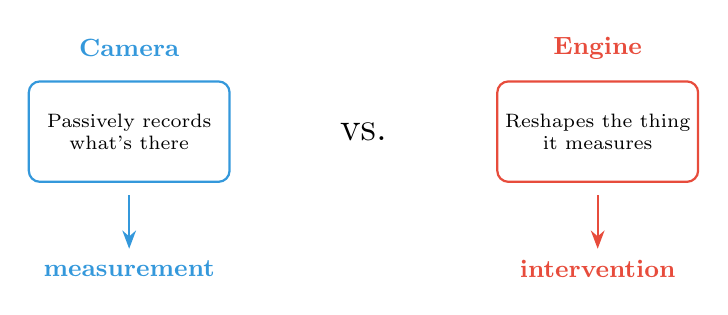
\begin{tikzpicture}[scale=0.85]
  % Camera
  \node[font=\small\bfseries,camera] at (2,3.5) {Camera};
  \draw[camera,thick,rounded corners] (0.5,1.5) rectangle (3.5,3);
  \node[font=\scriptsize,align=center] at (2,2.25) {Passively records\\what's there};
  \draw[camera,thick,-{Stealth}] (2,1.3) -- (2,0.5);
  \node[font=\small\bfseries,camera] at (2,0.2) {measurement};

  % vs
  \node[font=\Large] at (5.5,2.25) {vs.};

  % Engine
  \node[font=\small\bfseries,engine] at (9,3.5) {Engine};
  \draw[engine,thick,rounded corners] (7.5,1.5) rectangle (10.5,3);
  \node[font=\scriptsize,align=center] at (9,2.25) {Reshapes the thing\\it measures};
  \draw[engine,thick,-{Stealth}] (9,1.3) -- (9,0.5);
  \node[font=\small\bfseries,engine] at (9,0.2) {intervention};
\end{tikzpicture}
\end{center}
\end{frame}

%% --- SLIDE: Our claim ---
\begin{frame}{Our claim: benchmarks do the same thing}

\vspace{0.3em}

We argue that \textbf{ML benchmarks} operate exactly like Black-Scholes:

\vspace{0.5em}

\begin{enumerate}\setlength\itemsep{8pt}
  \item {\small A benchmark is introduced to \textbf{measure} model capability.}
  \item {\small Researchers optimize against it. Labs orient entire research programs around it.}
  \item {\small The benchmark stops measuring a pre-existing ability --- it starts \textbf{shaping} what gets built.}
  \item {\small Eventually the benchmark saturates, and the community recognizes it was measuring the wrong thing all along.}
\end{enumerate}

\vspace{0.5em}

{\small The benchmark is not a camera. It's an engine.}

\vspace{0.3em}
{\small We will now explore what that means --- for statistical validity, for proof standards in MI, and for peer review.}
\end{frame}

%% --- SLIDE: What performativity means ---
\begin{frame}{Three levels of performativity}

MacKenzie distinguishes how \emph{deeply} a model can reshape the world:

\vspace{0.5em}

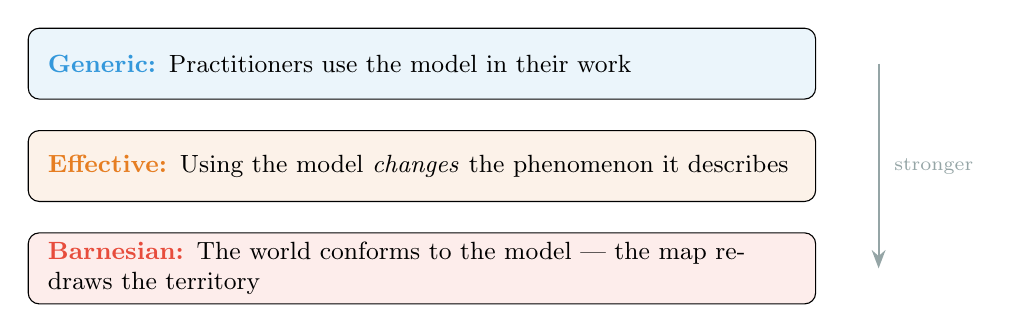
\begin{tikzpicture}[
  level/.style={draw,rounded corners,minimum width=10cm,minimum height=0.9cm,font=\small,align=left,text width=9.5cm},
]
  \node[level,fill=camera!10] (g) at (0,3.5) {\textbf{\textcolor{camera}{Generic:}} Practitioners use the model in their work};
  \node[level,fill=counter!10] (e) at (0,2.2) {\textbf{\textcolor{counter}{Effective:}} Using the model \emph{changes} the phenomenon it describes};
  \node[level,fill=engine!10] (b) at (0,0.9) {\textbf{\textcolor{engine}{Barnesian:}} The world conforms to the model --- the map redraws the territory};

  \draw[neutral,thick,-{Stealth}] (5.8,3.5) -- (5.8,0.9);
  \node[neutral,font=\scriptsize] at (6.5,2.2) {stronger};
\end{tikzpicture}

\vspace{0.5em}
Plus a failure mode: \textbf{\textcolor{counter}{counterperformativity}} --- when widespread adoption of the model causes the world to \emph{diverge} from its predictions.
\end{frame}

%% --- SLIDE: Concrete examples ---
\begin{frame}{Concrete examples of each level}

\begin{center}
{\small
\begin{tabular}{p{2.5cm}p{4.5cm}p{4.5cm}}
\toprule
\textbf{Level} & \textbf{Finance} & \textbf{ML} \\
\midrule
\textbf{\textcolor{camera}{Generic}} & Traders use Black-Scholes to price options & Researchers use ImageNet to evaluate models \\[6pt]
\textbf{\textcolor{counter}{Effective}} & Using the formula changes how options are priced & Optimising for ImageNet changes what architectures get built \\[6pt]
\textbf{\textcolor{engine}{Barnesian}} & Market prices converge to the formula's predictions & ``State of the art'' = ``best ImageNet score'' \\[6pt]
\textbf{\textcolor{fail}{Counter-}} & Gaussian copula creates the correlated risk it assumed away & ML evaluation inflates the false positives it aims to prevent \\
\bottomrule
\end{tabular}
}
\end{center}

\vspace{0.3em}
{\small The same instrument can be at different levels at different times. Black-Scholes was Barnesian in the 1980s and counterperformative in 1987.}
\end{frame}

%% --- SLIDE: The Gaussian copula ---
\begin{frame}{Counterperformativity: the Gaussian copula}

The clearest example of a model \textbf{destroying} what it assumed:

\vspace{0.5em}

\begin{enumerate}\setlength\itemsep{6pt}
  \item {\small David Li (2000) publishes the \href{https://en.wikipedia.org/wiki/Gaussian_copula}{\textbf{Gaussian copula}} formula for pricing mortgage-backed securities. Core assumption: defaults are only weakly correlated.}
  \item {\small Every major bank adopts it. Trillions of dollars of CDOs are priced using this one model.}
  \item {\small Because everyone uses the same model with the same assumption, they all hold the same risks. The \textbf{actual} correlation between defaults increases.}
  \item {\small In 2007--08, correlated defaults cascade through the system. The model's assumption of low correlation \textbf{created} the high correlation that broke it.}
\end{enumerate}

\vspace{0.5em}
{\small The safety model generated the danger it was supposed to prevent. We argue the same structure operates in ML benchmarks.}
\end{frame}

%% --- SLIDE: Mapping to ML ---
\begin{frame}{Mapping this to ML benchmarks}
\begin{columns}[T]
\begin{column}{0.48\textwidth}
\centering
{\small \textbf{Financial models}}

\vspace{0.3em}
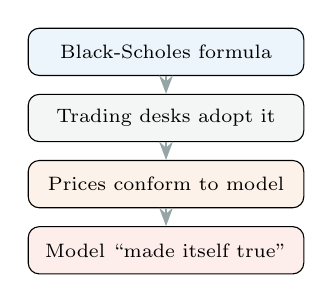
\begin{tikzpicture}[scale=0.7,
  box/.style={draw,rounded corners,fill=#1!10,minimum width=3.5cm,minimum height=0.6cm,font=\scriptsize},
]
  \node[box=camera] (bs) at (0,3) {Black-Scholes formula};
  \node[box=neutral] (td) at (0,1.8) {Trading desks adopt it};
  \node[box=counter] (pr) at (0,0.6) {Prices conform to model};
  \node[box=engine] (cr) at (0,-0.6) {Model ``made itself true''};

  \draw[-{Stealth},thick,neutral] (bs) -- (td);
  \draw[-{Stealth},thick,neutral] (td) -- (pr);
  \draw[-{Stealth},thick,neutral] (pr) -- (cr);
\end{tikzpicture}
\end{column}
\begin{column}{0.48\textwidth}
\centering
{\small \textbf{ML benchmarks}}

\vspace{0.3em}
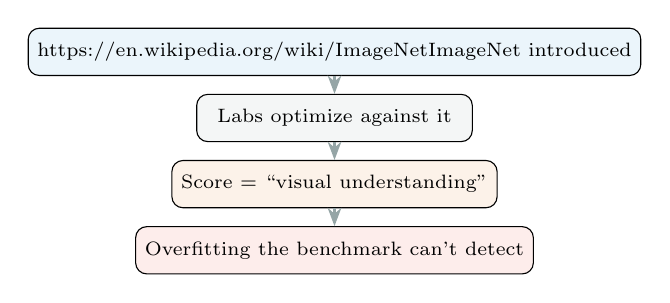
\begin{tikzpicture}[scale=0.7,
  box/.style={draw,rounded corners,fill=#1!10,minimum width=3.5cm,minimum height=0.6cm,font=\scriptsize},
]
  \node[box=camera] (im) at (0,3) {\href{https://en.wikipedia.org/wiki/ImageNet}{ImageNet} introduced};
  \node[box=neutral] (op) at (0,1.8) {Labs optimize against it};
  \node[box=counter] (df) at (0,0.6) {Score $=$ ``visual understanding''};
  \node[box=engine] (ov) at (0,-0.6) {Overfitting the benchmark can't detect};

  \draw[-{Stealth},thick,neutral] (im) -- (op);
  \draw[-{Stealth},thick,neutral] (op) -- (df);
  \draw[-{Stealth},thick,neutral] (df) -- (ov);
\end{tikzpicture}
\end{column}
\end{columns}

\vspace{0.5em}
{\small The channels are different (trading desks vs.\ conference leaderboards), but the dynamic is the same: the instrument reshapes what it measures.}
\end{frame}

%% --- SLIDE: The analogy is not exact ---
\begin{frame}{Where the analogy breaks (and where it holds)}

\begin{columns}[T]
\begin{column}{0.48\textwidth}
\textbf{Where it holds}
\begin{itemize}\setlength\itemsep{4pt}
  \item {\small The instrument reshapes the thing it claims to measure}
  \item {\small Adoption is driven by institutional incentives, not just technical merit}
  \item {\small The community treats the model's output as ground truth}
  \item {\small Failure modes emerge from collective adoption, not individual misuse}
\end{itemize}
\end{column}
\begin{column}{0.48\textwidth}
\textbf{Where it differs}
\begin{itemize}\setlength\itemsep{4pt}
  \item {\small No single formula --- many benchmarks, loosely coordinated}
  \item {\small No direct financial feedback loop (prices don't clear)}
  \item {\small We claim \textbf{effective} performativity, not Barnesian --- benchmarks reshape research priorities, not reality itself}
  \item {\small The ``crash'' is slow replacement, not a sudden crisis}
\end{itemize}
\end{column}
\end{columns}

\vspace{0.5em}
{\small We're not claiming ML $=$ finance. We're claiming the \textbf{structure} is the same: an instrument presented as a camera that functions as an engine.}
\end{frame}

%% --- SLIDE: The lifecycle ---
\begin{frame}{The benchmark lifecycle}
\begin{columns}[T]
\begin{column}{0.48\textwidth}
{\small Every benchmark goes through four phases:}

\vspace{0.3em}
\begin{enumerate}\setlength\itemsep{2pt}
  \item {\small \textbf{\textcolor{camera}{Camera.}} Introduced as a measurement. Passively records model performance.}
  \item {\small \textbf{Adoption.} Researchers optimize against it. Leaderboards emerge. Score $=$ the capability.}
  \item {\small \textbf{\textcolor{counter}{Saturation.}} Optimisation changes what models are built. The benchmark reshapes training, data, architecture.}
  \item {\small \textbf{\textcolor{engine}{Crash.}} Benchmark is saturated or recognized as measuring the wrong thing. Replaced. Cycle restarts.}
\end{enumerate}
\end{column}
\begin{column}{0.50\textwidth}
\centering
\vspace{-0.5em}
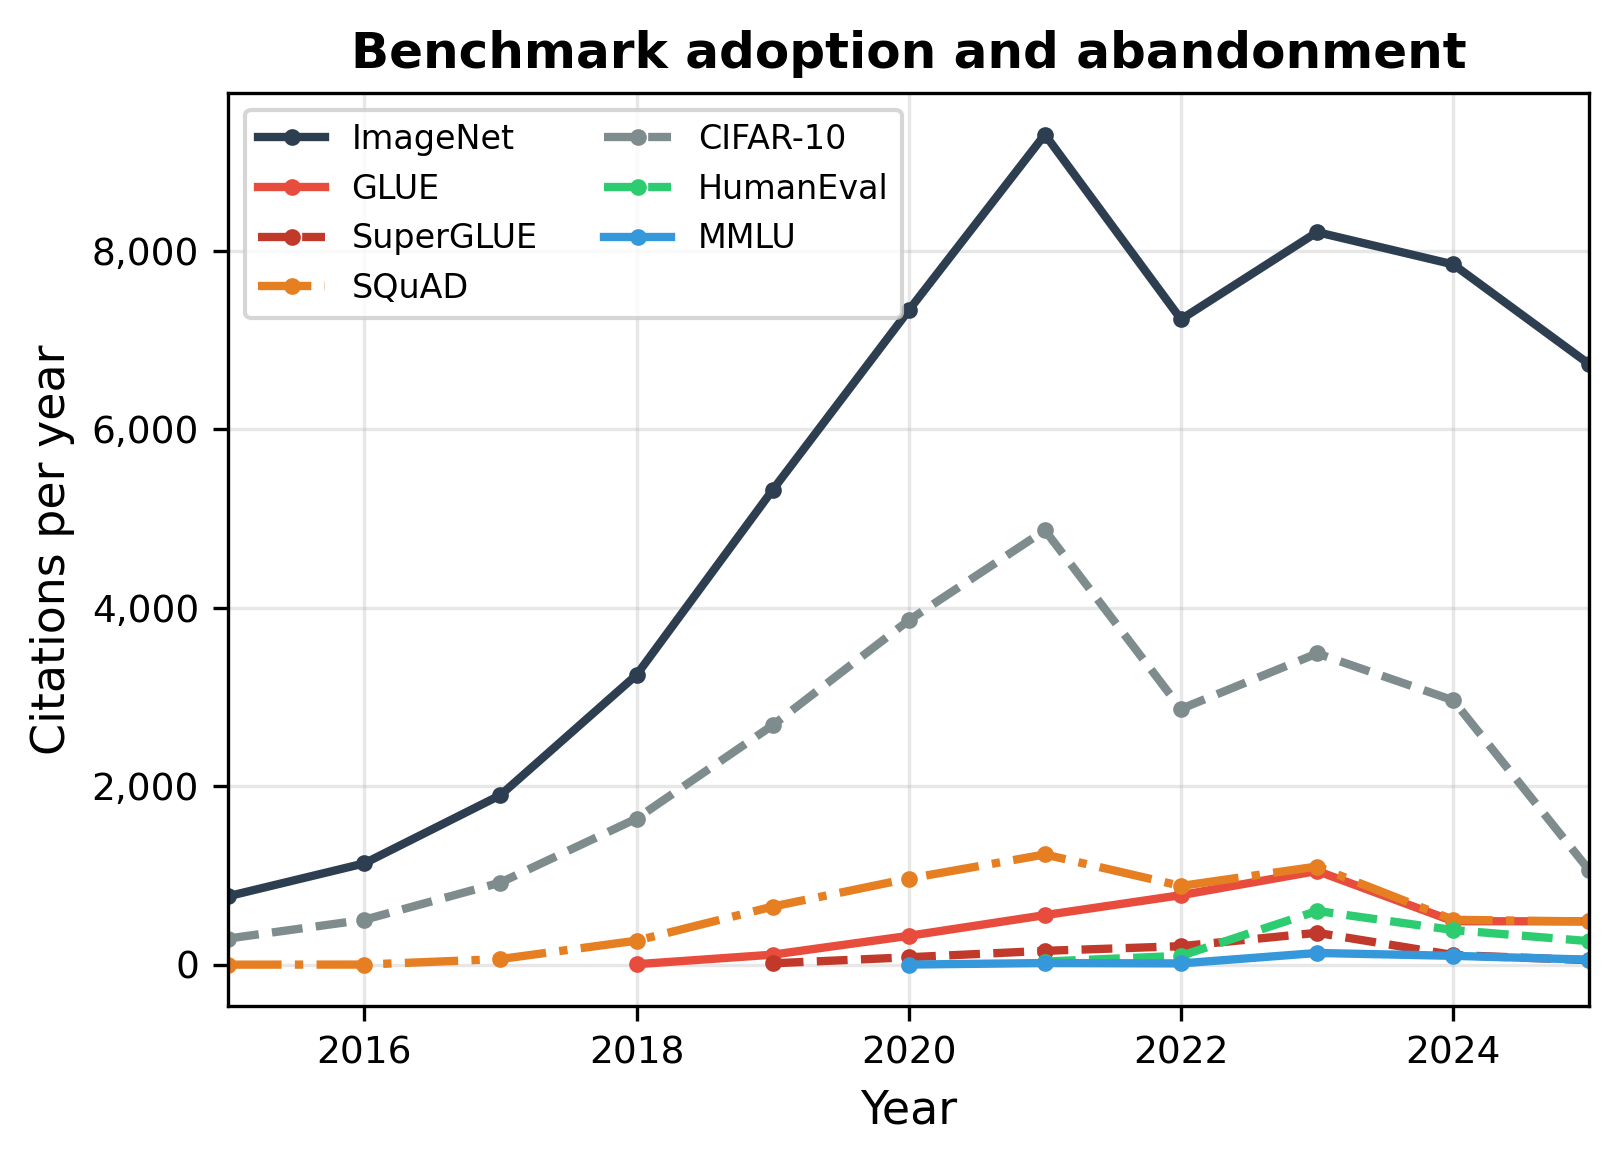
\includegraphics[width=\linewidth]{fig_lifecycle_single.png}

\vspace{0.3em}
{\scriptsize\raggedright NLP benchmarks (GLUE, SuperGLUE) crash in 3--5 years.\\Vision benchmarks (ImageNet) persist as cultural institutions.\par}
\end{column}
\end{columns}
\end{frame}

%% --- SLIDE: NLP speed ---
\begin{frame}{NLP benchmarks crash fast}

\begin{center}
{\small
\begin{tabular}{lccrc}
\toprule
\textbf{Benchmark} & \textbf{Domain} & \textbf{Introduced} & \textbf{Peak cites/yr} & \textbf{Decline to 2024} \\
\midrule
\href{https://arxiv.org/abs/1804.07461}{GLUE} & NLP & 2018 & 1,052 & \textcolor{fail}{$-$54\%} \\
\href{https://arxiv.org/abs/1905.00537}{SuperGLUE} & NLP & 2019 & 359 & \textcolor{fail}{$-$69\%} \\
\href{https://arxiv.org/abs/1606.05250}{SQuAD} & NLP & 2016 & 1,237 & \textcolor{fail}{$-$59\%} \\
\midrule
\href{https://en.wikipedia.org/wiki/ImageNet}{ImageNet} & Vision & 2009 & 9,305 & \textcolor{pass}{$-$16\%} \\
\href{https://en.wikipedia.org/wiki/CIFAR-10}{CIFAR-10} & Vision & 2009 & 4,870 & \textcolor{counter}{$-$39\%} \\
\bottomrule
\end{tabular}
}
\end{center}

\vspace{0.3em}
{\small \textbf{Key pattern:} NLP benchmarks are abandoned when models saturate them --- not when the underlying capability is ``solved.''}

\vspace{0.2em}
{\small GLUE wasn't replaced because language understanding was solved. It was replaced because BERT-scale models maxed out the score and the community needed something harder.}

\vspace{0.2em}
{\small The benchmark tracks \textbf{social utility} --- the ability to rank models.}
\end{frame}


%% ============================================================
%% PART 2: PROOF CULTURES
%% ============================================================

\begin{frame}[plain]
\vfill
\begin{center}
  \setlength{\fboxrule}{2.5pt}%
  \fcolorbox{black}{white}{\parbox{0.7\textwidth}{\centering\vspace{0.8em}
    {\Large\bfseries Part 2}\\[0.5em]
    {\large Proof cultures and the denominator problem}
  \vspace{0.8em}}}
\end{center}
\vfill
\end{frame}

%% --- SLIDE: What is MI? ---
\begin{frame}{What is mechanistic interpretability?}

The goal: understand \textbf{how} neural networks compute, not just \emph{what} they compute.

\vspace{0.5em}

\begin{columns}[T]
\begin{column}{0.48\textwidth}
\textbf{Standard ML evaluation}
\begin{itemize}\setlength\itemsep{3pt}
  \item {\small Run model on test set}
  \item {\small Report accuracy, F1, BLEU, etc.}
  \item {\small The model is a \textbf{black box}}
\end{itemize}

\vspace{0.3em}
{\small This tells you \emph{what} the model does, but not \emph{why} or \emph{how}.}
\end{column}
\begin{column}{0.48\textwidth}
\textbf{Mechanistic interpretability}
\begin{itemize}\setlength\itemsep{3pt}
  \item {\small Open up the model}
  \item {\small Identify internal components (features, circuits, causal variables)}
  \item {\small Explain \textbf{how it works}}
\end{itemize}

\vspace{0.3em}
{\small This is a young field. There is not yet broad agreement on what counts as evidence.}
\end{column}
\end{columns}

\vspace{0.5em}
{\small That disagreement is the subject of Part 2.}
\end{frame}

%% --- SLIDE: What is a proof culture? ---
\begin{frame}{What is a ``proof culture''?}
\begin{columns}[T]
\begin{column}{0.55\textwidth}
{\small MacKenzie studied \href{https://mitpress.mit.edu/9780262632959/mechanizing-proof/}{formal verification}: what counts as a valid ``proof'' that a computer system is correct.}

\vspace{0.3em}
{\small He found that \textbf{logicians}, \textbf{mathematicians}, and \textbf{engineers} accepted different kinds of arguments as proof. The boundary was shaped by funding and institutional authority, not just by logic.}

\vspace{0.3em}
{\small The same thing is happening in mechanistic interpretability. Three communities are trying to answer the same question --- ``how do neural networks compute?'' --- using \textbf{incompatible evidence standards}.}
\end{column}
\begin{column}{0.42\textwidth}
\centering
\vspace{0.5em}
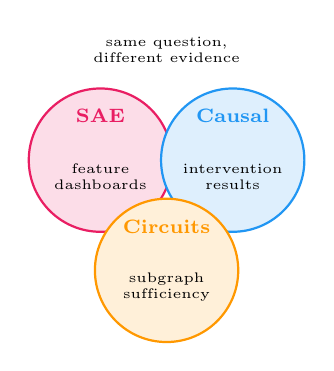
\begin{tikzpicture}[scale=0.7]
  % Three overlapping but separate circles
  \fill[sae!15] (-1.2,1.5) circle (1.3);
  \draw[sae,thick] (-1.2,1.5) circle (1.3);
  \node[sae,font=\scriptsize\bfseries] at (-1.2,2.3) {SAE};
  \node[font=\tiny,align=center] at (-1.2,1.2) {feature\\dashboards};

  \fill[causal!15] (1.2,1.5) circle (1.3);
  \draw[causal,thick] (1.2,1.5) circle (1.3);
  \node[causal,font=\scriptsize\bfseries] at (1.2,2.3) {Causal};
  \node[font=\tiny,align=center] at (1.2,1.2) {intervention\\results};

  \fill[circuits!15] (0,-0.5) circle (1.3);
  \draw[circuits,thick] (0,-0.5) circle (1.3);
  \node[circuits,font=\scriptsize\bfseries] at (0,0.3) {Circuits};
  \node[font=\tiny,align=center] at (0,-0.8) {subgraph\\sufficiency};

  % No overlap between SAE and Causal
  \node[font=\tiny,align=center] at (0,3.5) {same question,\\different evidence};
\end{tikzpicture}
\end{column}
\end{columns}
\end{frame}

%% --- SLIDE: Three communities ---
\begin{frame}{Three communities, three evidence standards}

\begin{columns}[T]
\begin{column}{0.32\textwidth}
\centering
\textbf{\textcolor{sae}{Sparse Autoencoders}}

\vspace{0.3em}
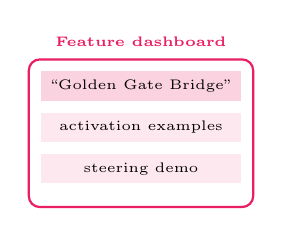
\begin{tikzpicture}[scale=0.75]
  \draw[sae,thick,rounded corners] (0,0) rectangle (3.8,2.5);
  \node[font=\tiny\bfseries,sae] at (1.9,2.8) {Feature dashboard};
  \fill[sae!20] (0.2,1.8) rectangle (3.6,2.3);
  \node[font=\tiny] at (1.9,2.05) {``Golden Gate Bridge''};
  \fill[sae!10] (0.2,1.1) rectangle (3.6,1.6);
  \node[font=\tiny] at (1.9,1.35) {activation examples};
  \fill[sae!10] (0.2,0.4) rectangle (3.6,0.9);
  \node[font=\tiny] at (1.9,0.65) {steering demo};
\end{tikzpicture}

\vspace{0.3em}
{\scriptsize Valid if features are \textbf{interpretable} and monosemantic.}
\end{column}
\begin{column}{0.32\textwidth}
\centering
\textbf{\textcolor{causal}{Causal Abstraction}}

\vspace{0.3em}
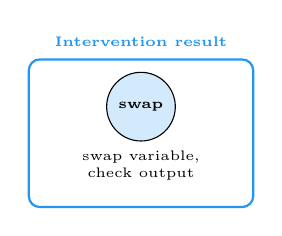
\begin{tikzpicture}[scale=0.75]
  \draw[causal,thick,rounded corners] (0,0) rectangle (3.8,2.5);
  \node[font=\tiny\bfseries,causal] at (1.9,2.8) {Intervention result};
  \node[draw,circle,fill=causal!20,minimum size=0.6cm,font=\tiny\bfseries] (sw) at (1.9,1.7) {swap};
  \node[font=\tiny,align=center] at (1.9,0.7) {swap variable,\\check output};
\end{tikzpicture}

\vspace{0.3em}
{\scriptsize Valid if \textbf{interventions} produce predicted effects.}
\end{column}
\begin{column}{0.32\textwidth}
\centering
\textbf{\textcolor{circuits}{Circuit Discovery}}

\vspace{0.3em}
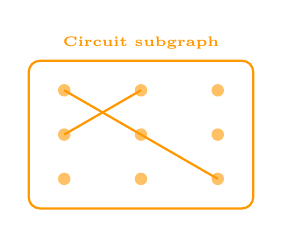
\begin{tikzpicture}[scale=0.75]
  \draw[circuits,thick,rounded corners] (0,0) rectangle (3.8,2.5);
  \node[font=\tiny\bfseries,circuits] at (1.9,2.8) {Circuit subgraph};
  \foreach \y in {0.5, 1.25, 2.0} {
    \fill[circuits!60] (0.6,\y) circle (3pt);
    \fill[circuits!60] (1.9,\y) circle (3pt);
    \fill[circuits!60] (3.2,\y) circle (3pt);
  }
  \draw[circuits,thick] (0.6,2.0) -- (1.9,1.25);
  \draw[circuits,thick] (1.9,1.25) -- (3.2,0.5);
  \draw[circuits,thick] (0.6,1.25) -- (1.9,2.0);
\end{tikzpicture}

\vspace{0.3em}
{\scriptsize Valid if the circuit is \textbf{necessary and sufficient} for the behavior.}
\end{column}
\end{columns}

\vspace{0.5em}
{\small These are not interchangeable. A feature dashboard would not satisfy a causal abstraction reviewer; an intervention result would not satisfy a circuits reviewer. Each community has its own ``what counts as evidence.''}
\end{frame}

%% --- SLIDE: Subfields don't cite each other ---
\begin{frame}{Subfields don't cite each other}
\begin{columns}[T]
\begin{column}{0.55\textwidth}
{\small We analyzed citation links among 688 MI papers (209 SAE, 40 Causal, 128 Circuits, 311 general).}

\vspace{0.5em}
{\small
\begin{tabular}{lccc}
\toprule
\textbf{From $\backslash$ To} & \textbf{\textcolor{sae}{SAE}} & \textbf{\textcolor{causal}{Causal}} & \textbf{\textcolor{circuits}{Circuits}} \\
\midrule
\textcolor{sae}{SAE} & 326 & \textcolor{fail}{\textbf{14}} & 45 \\
\textcolor{causal}{Causal} & \textcolor{fail}{\textbf{9}} & 63 & 16 \\
\textcolor{circuits}{Circuits} & 38 & 62 & 157 \\
\bottomrule
\end{tabular}
}

\vspace{0.5em}
{\small SAE $\leftrightarrow$ Causal: \textbf{23 cross-citations} across 16,720 possible directed pairs.}

\vspace{0.3em}
{\small That's \textbf{0.14\% density}. Both communities cite circuits literature, but barely cite each other.}
\end{column}
\begin{column}{0.42\textwidth}
\centering
\vspace{0.5em}
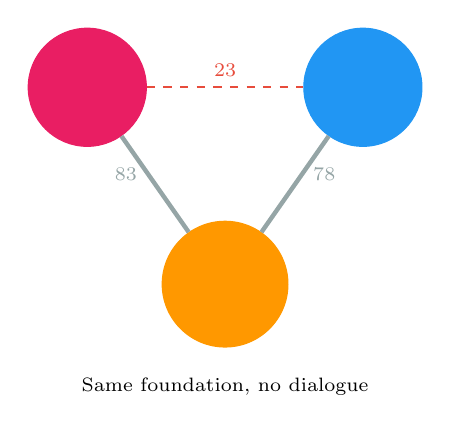
\begin{tikzpicture}[scale=1.0]
  % Three nodes
  \node[draw,circle,fill=sae!20,minimum size=1.5cm,font=\small\bfseries,sae] (s) at (0,3) {SAE};
  \node[draw,circle,fill=causal!20,minimum size=1.5cm,font=\small\bfseries,causal] (c) at (3.5,3) {Causal};
  \node[draw,circle,fill=circuits!20,minimum size=1.5cm,font=\small\bfseries,circuits] (ci) at (1.75,0.5) {Circuits};

  % Heavy edges to circuits
  \draw[neutral,ultra thick] (s) -- node[font=\scriptsize,left,pos=0.4] {83} (ci);
  \draw[neutral,ultra thick] (c) -- node[font=\scriptsize,right,pos=0.4] {78} (ci);

  % Thin edge between SAE and Causal
  \draw[fail,dashed,thick] (s) -- node[font=\scriptsize,above] {23} (c);

  \node[font=\scriptsize,align=center] at (1.75,-0.8) {Same foundation, no dialogue};
\end{tikzpicture}
\end{column}
\end{columns}
\end{frame}

%% --- SLIDE: The denominator problem ---
\begin{frame}{The denominator problem}
\begin{columns}[T]
\begin{column}{0.55\textwidth}
{\small An SAE trains a dictionary of $N$ features. The researcher analyzes them and ultimately chooses to display the $k$ most interesting ones.}

\vspace{0.3em}
{\small This is a multiple hypothesis test with $m \geq N$. None of the papers we audited corrects for it.}

\vspace{0.5em}
\textbf{The worked example:}\\
{\small \href{https://transformer-circuits.pub/2024/scaling-monosemanticity/}{Templeton et al.\ (2024)} trained \textbf{34 million} features on Claude 3 Sonnet. They showed $\sim$10 in detail.}

\vspace{0.3em}
{\small Selection ratio: \textbf{3.4 million to one}.}

\vspace{0.3em}
{\small If even 0.01\% of features are spuriously interpretable, that's \textbf{3,400 false positives} --- dwarfing the 10 shown.}
\end{column}
\begin{column}{0.48\textwidth}
\centering
\vspace{0.3em}
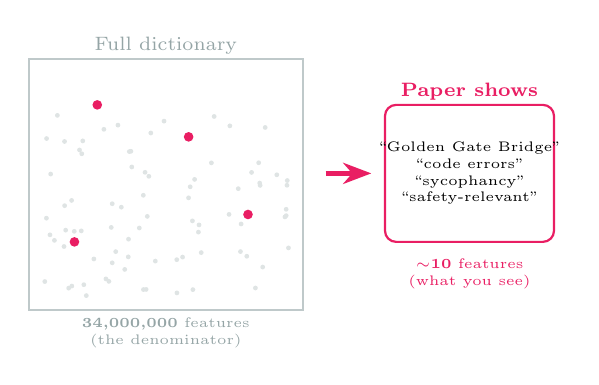
\begin{tikzpicture}[scale=0.58]
  % Full dictionary
  \draw[thick,neutral!60] (0,0) rectangle (6,5.5);
  \node[font=\scriptsize,neutral] at (3,5.8) {Full dictionary};

  % Many many dots (the denominator)
  \foreach \i in {1,...,80} {
    \pgfmathsetmacro{\x}{0.3+5.4*rnd}
    \pgfmathsetmacro{\y}{0.3+4.0*rnd}
    \fill[neutral!30] (\x,\y) circle (1.5pt);
  }

  % A few highlighted (the shown ones)
  \fill[sae] (1.5,4.5) circle (3pt);
  \fill[sae] (3.5,3.8) circle (3pt);
  \fill[sae] (4.8,2.1) circle (3pt);
  \fill[sae] (1.0,1.5) circle (3pt);

  % Arrow
  \draw[sae,ultra thick,-{Stealth}] (6.5,3) -- (7.5,3);

  % Dashboard
  \draw[sae,thick,rounded corners] (7.8,1.5) rectangle (11.5,4.5);
  \node[font=\scriptsize\bfseries,sae] at (9.65,4.8) {Paper shows};
  \node[font=\tiny,align=center] at (9.65,3) {``Golden Gate Bridge''\\``code errors''\\``sycophancy''\\``safety-relevant''};

  % Labels
  \node[font=\tiny,neutral,align=center] at (3,-0.5) {\textbf{34,000,000} features\\(the denominator)};
  \node[font=\tiny,sae,align=center] at (9.65,0.8) {\textbf{$\sim$10} features\\(what you see)};
\end{tikzpicture}
\end{column}
\end{columns}
\end{frame}

%% --- SLIDE: The practitioner's funnel ---
\begin{frame}{The practitioner's funnel}

{\small Even outside MI, the denominator is invisible. A typical ML project:}

\vspace{0.5em}

\begin{center}
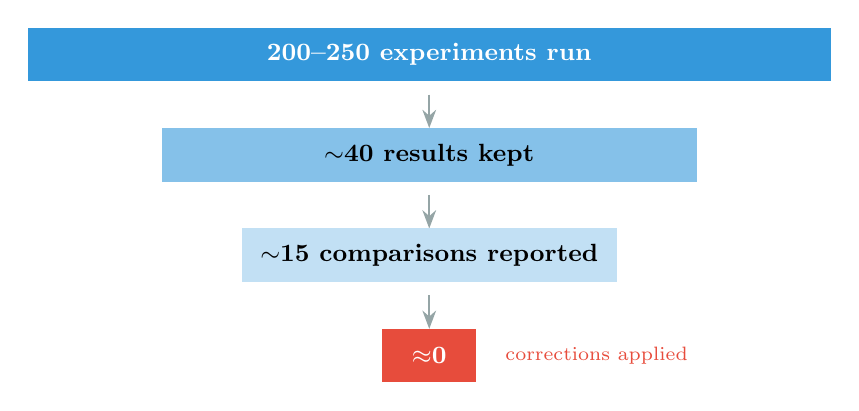
\begin{tikzpicture}[scale=0.85]
  % Funnel bars
  \fill[camera] (-1,4.5) rectangle (11,5.3);
  \node[font=\small\bfseries,white] at (5,4.9) {200--250 experiments run};

  \draw[-{Stealth},thick,neutral] (5,4.3) -- (5,3.8);

  \fill[camera!60] (1,3.0) rectangle (9,3.8);
  \node[font=\small\bfseries] at (5,3.4) {$\sim$40 results kept};

  \draw[-{Stealth},thick,neutral] (5,2.8) -- (5,2.3);

  \fill[camera!30] (2.2,1.5) rectangle (7.8,2.3);
  \node[font=\small\bfseries] at (5,1.9) {$\sim$15 comparisons reported};

  \draw[-{Stealth},thick,neutral] (5,1.3) -- (5,0.8);

  \fill[engine] (4.3,0) rectangle (5.7,0.8);
  \node[font=\small\bfseries,white] at (5,0.4) {$\approx$0};
  \node[font=\scriptsize,engine] at (7.5,0.4) {corrections applied};
\end{tikzpicture}
\end{center}

\vspace{0.3em}
{\small The paper reports 15 comparisons. The reviewer sees 15. The reader sees 15. But 200+ were run. \textbf{The denominator is invisible by default.}}
\end{frame}

%% --- SLIDE: Multiple comparisons intuition ---
\begin{frame}{The multiple comparisons problem}

A simple thought experiment:

\vspace{0.3em}

{\small Flip a fair coin 20 times. The chance of getting heads at least once is not $5\%$ --- it's $\mathbf{64\%}$.}

\vspace{0.3em}

{\small Now imagine running 20 experiments, each with a 5\% false positive rate. The chance that \emph{at least one} gives a false positive is also 64\%.}

\vspace{0.3em}

\begin{center}

\begin{tikzpicture}[scale=0.85]
  \foreach \i in {1,...,20} {
    \pgfmathsetmacro{\x}{(\i-1)*0.55}
    \fill[camera!30] (\x,0) rectangle (\x+0.4,0.8);
  }
  \fill[engine] (0.55*6,0) rectangle (0.55*6+0.4,0.8);
  \node[font=\scriptsize,engine,above] at (0.55*6+0.2,0.9) {false positive};
  \node[font=\scriptsize,neutral] at (5.5,-0.4) {20 independent tests at $\alpha = 0.05$};
\end{tikzpicture}
\end{center}

\vspace{0.2em}

{\small This is well understood in medicine and genetics. Researchers routinely correct for it. In ML, almost nobody does.}
\end{frame}

%% --- SLIDE: Metric 1: FWER ---
\begin{frame}{Metric 1: \href{https://en.wikipedia.org/wiki/Family-wise_error_rate}{Family-wise error rate} (FWER)}

{\small The probability that \emph{at least one} of your comparisons is a false positive.}

\vspace{0.5em}

\begin{center}
$\text{FWER} = 1 - (1 - \alpha)^m$
\end{center}

\vspace{0.5em}

{\small At $\alpha = 0.05$:}

\vspace{0.3em}

{\small
\begin{tabular}{lrl}
\toprule
\textbf{Comparisons ($m$)} & \textbf{FWER} & \\
\midrule
5 & 23\% & (typical single experiment) \\
20 & 64\% & (typical paper) \\
100 & 99.4\% & (hyperparameter search) \\
1,000 & $\approx$100\% & (architecture search) \\
\bottomrule
\end{tabular}
}

\vspace{0.5em}

{\small With enough comparisons, finding ``significant'' results is guaranteed by chance alone. Controlling FWER means ensuring this probability stays below $\alpha$.}
\end{frame}

%% --- SLIDE: Metric 2: FDR ---
\begin{frame}{Metric 2: \href{https://en.wikipedia.org/wiki/False_discovery_rate}{False discovery rate} (FDR)}

{\small The expected \emph{proportion} of false positives among your claimed discoveries.}

\vspace{0.5em}

\begin{center}
$\text{FDR} = \mathbb{E}\left[\frac{\text{false positives}}{\text{total rejections}}\right]$
\end{center}

\vspace{0.5em}

{\small At $q = 0.05$, no matter how many tests you run:}

\vspace{0.3em}

{\small
\begin{tabular}{lrrl}
\toprule
\textbf{Tests} & \textbf{Discoveries} & \textbf{Expected false} & \\
\midrule
20 & 4 & $\sim$0.2 & (5\% of 4) \\
100 & 20 & $\sim$1 & (5\% of 20) \\
1,000 & 50 & $\sim$2.5 & (5\% of 50) \\
10,000 & 200 & $\sim$10 & (5\% of 200) \\
\bottomrule
\end{tabular}
}

\vspace{0.5em}

{\small FDR scales with discoveries, not total tests. It's less strict than FWER --- you accept some false positives --- but you find far more real effects. The tradeoff: you know $\sim$5\% of your results are wrong, but not \emph{which} 5\%.}
\end{frame}

%% --- SLIDE: What is Bonferroni? ---
\begin{frame}{Control 1: \href{https://en.wikipedia.org/wiki/Bonferroni_correction}{Bonferroni correction} (1936)}

The simplest fix has existed since 1936:

\vspace{0.5em}

\begin{center}
{\large If you run $m$ comparisons, divide your significance threshold by $m$.}

\vspace{0.5em}

$$\alpha_{\text{corrected}} = \frac{\alpha}{m} = \frac{0.05}{m}$$
\end{center}

\vspace{0.5em}

{\small
\begin{tabular}{lccc}
\toprule
\textbf{Field} & \textbf{Typical $m$} & \textbf{Corrected $\alpha$} & \textbf{Correction used?} \\
\midrule
Clinical trials & 3--5 & 0.01 & Always (FDA requires it) \\
Genomics (GWAS) & 1,000,000 & $5 \times 10^{-8}$ & Always \\
Psychology & 5--20 & 0.003--0.01 & Usually \\
ML (standard) & 100--1,000+ & would be $10^{-4}$ & Almost never \\
ML (MI/SAEs) & 1,000--34,000,000 & would be $10^{-9}$ & Never \\
\bottomrule
\end{tabular}
}

\vspace{0.5em}
{\small Bonferroni is conservative --- it assumes all tests are independent. This makes it safe but often too strict.}
\end{frame}

%% --- SLIDE: Holm correction ---
\begin{frame}{Control 2: \href{https://en.wikipedia.org/wiki/Holm\%E2\%80\%93Bonferroni_method}{Holm--Bonferroni method} (1979)}

A strictly more powerful version of Bonferroni:

\vspace{0.5em}

\begin{enumerate}\setlength\itemsep{6pt}
  \item {\small Sort your $m$ p-values from smallest to largest: $p_{(1)} \leq p_{(2)} \leq \cdots \leq p_{(m)}$}
  \item {\small Compare each $p_{(i)}$ against a \emph{different} threshold: $\frac{\alpha}{m - i + 1}$}
  \item {\small Reject from the smallest up, stop at the first non-rejection}
\end{enumerate}

\vspace{0.5em}

\begin{center}
{\small
\begin{tabular}{lccc}
\toprule
\textbf{Rank} & \textbf{P-value} & \textbf{Bonferroni threshold} & \textbf{Holm threshold} \\
\midrule
1st & 0.003 & 0.05/5 = 0.010 & 0.05/5 = 0.010 \\
2nd & 0.009 & 0.05/5 = 0.010 & 0.05/4 = 0.0125 \\
3rd & 0.02 & 0.05/5 = 0.010 & 0.05/3 = 0.017 \\
\bottomrule
\end{tabular}
}
\end{center}

\vspace{0.3em}
{\small Holm rejects \emph{at least} as many hypotheses as Bonferroni. It is uniformly more powerful while still controlling FWER. There is no reason to use Bonferroni over Holm.}
\end{frame}

%% --- SLIDE: Benjamini-Hochberg ---
\begin{frame}{Control 3: \href{https://en.wikipedia.org/wiki/False_discovery_rate\#Benjamini\%E2\%80\%93Hochberg_procedure}{Benjamini--Hochberg procedure} (1995)}

A different philosophy: control the \textbf{false discovery rate} (FDR) instead of FWER.

\vspace{0.5em}

{\small
\textbf{FWER}: probability of \emph{any} false positive $\leq \alpha$\\
\textbf{FDR}: expected \emph{proportion} of false positives among rejections $\leq q$
}

\vspace{0.5em}

\begin{enumerate}\setlength\itemsep{6pt}
  \item {\small Sort p-values: $p_{(1)} \leq \cdots \leq p_{(m)}$}
  \item {\small Find the largest $k$ such that $p_{(k)} \leq \frac{k}{m} \cdot q$}
  \item {\small Reject all hypotheses $1, \ldots, k$}
\end{enumerate}

\vspace{0.5em}

{\small This is much less conservative than Bonferroni/Holm. If you run 1,000 tests at $q = 0.05$, you accept that $\sim$50 of your ``discoveries'' may be false --- but you find far more real effects.}

\vspace{0.3em}
{\small Widely used in genomics (thousands of genes tested simultaneously). Almost never used in ML.}
\end{frame}

%% --- SLIDE: Which correction when? ---
\begin{frame}{Which correction to use?}

\vspace{0.3em}

{\small
\begin{tabular}{lp{4cm}p{4.5cm}}
\toprule
\textbf{Method} & \textbf{Controls} & \textbf{Best for} \\
\midrule
Bonferroni & FWER (strictest) & Very few tests; need zero false positives (clinical trials) \\[4pt]
Holm & FWER (uniformly better) & Same situations as Bonferroni --- strictly dominates it \\[4pt]
Benjamini--Hochberg & FDR (more lenient) & Many tests; some false positives acceptable (screening, genomics) \\
\bottomrule
\end{tabular}
}

\vspace{0.8em}

{\small \textbf{For ML experiments} (5--20 reported comparisons): Holm is the obvious default. It costs nothing, requires no assumptions beyond independence, and is trivial to implement.}

\vspace{0.5em}

{\small \textbf{For MI/SAE feature selection} (thousands--millions of candidates): BH-style FDR control is more appropriate, since FWER becomes impossibly strict at that scale.}

\vspace{0.5em}

{\small \textbf{Current practice in ML}: almost none of them. The field reports raw p-values --- or more commonly, no p-values at all.}
\end{frame}

%% --- SLIDE: What other fields require ---
\begin{frame}{What other fields require}

\vspace{0.3em}

{\small
\begin{tabular}{lp{5.5cm}l}
\toprule
\textbf{Field} & \textbf{Requirement} & \textbf{Enforced by} \\
\midrule
Clinical trials & Pre-registered correction (usually Bonferroni or Hochberg) & FDA / EMA (law) \\[4pt]
Genomics (GWAS) & Genome-wide threshold $5 \times 10^{-8}$ or BH-FDR & Journal policy \\[4pt]
Psychology & Correction mandatory since replication crisis & APA guidelines \\[4pt]
Neuroscience & Cluster-level FWE or FDR for imaging & Field norm \\[4pt]
\bottomrule
\end{tabular}
}

\vspace{0.8em}

{\small These aren't suggestions --- in clinical trials, submitting results without pre-specified multiplicity adjustment is grounds for regulatory rejection. The FDA has mandated this since 1998.}

\vspace{0.5em}

{\small ML has no equivalent authority, no pre-registration norm, and no review checklist that asks ``how many comparisons did you actually run?''}
\end{frame}


%% --- SLIDE: What counts as a comparison? ---
\begin{frame}{What counts as a ``comparison'' in ML?}

This is the key question. In ML, comparisons are often \textbf{implicit}:

\vspace{0.5em}

\begin{itemize}\setlength\itemsep{5pt}
  \item {\small Every hyperparameter setting you tried}
  \item {\small Every architecture variant you tested}
  \item {\small Every random seed you ran (and kept the best)}
  \item {\small Every baseline you compared against}
  \item {\small Every dataset split you evaluated on}
  \item {\small Every feature you looked at and decided to show}
\end{itemize}

\vspace{0.5em}

{\small A paper reporting ``5 experiments'' may have actually run 200+. The \textbf{denominator} --- the total number of comparisons --- is invisible to the reader.}

\vspace{0.3em}
{\small This is not fraud. It's the default workflow. But it has statistical consequences.}
\end{frame}

%% --- SLIDE: Why this matters ---


%% --- SLIDE: FWER in MI: the scale ---
\begin{frame}{The scale of the problem in MI}

{\small Implicit comparison counts from real MI papers:}

\vspace{0.5em}

{\small
\begin{tabular}{lrrl}
\toprule
\textbf{Paper} & \textbf{Comparisons ($m$)} & \textbf{FWER} & \textbf{Corrected?} \\
\midrule
Typical ML paper & 100--500 & $>$99\% & No \\
IOI circuit (Wang+ 2022) & $\sim$1,000 & $\approx$100\% & No \\
SAEBench (Karvonen+ 2025) & $\sim$10,000 & $\approx$100\% & No \\
Scaling Monosemanticity (2024) & 34,000,000 & $\approx$100\% & No \\
\bottomrule
\end{tabular}
}

\vspace{0.8em}

{\small Every one of these papers reports ``interesting'' features or circuits. At these scales, finding interesting-looking results is \emph{guaranteed} --- even in random noise.}

\vspace{0.5em}

{\small The question is not whether SAE features look interpretable. It's whether the false positives are a problem.}
\end{frame}


%% --- SLIDE: How genomics solved this ---
\begin{frame}{How genomics solved this}

{\small Genome-wide association studies (GWAS) test $\sim$1,000,000 genetic variants per study. Same scale as MI. Their solution (standardized since $\sim$2005):}

\vspace{0.3em}

\begin{enumerate}\setlength\itemsep{3pt}
  \item {\small \textbf{Pre-register} the number of tests before looking at data}
  \item {\small Apply BH-FDR at $q = 0.05$ for discovery (screening phase)}
  \item {\small Replicate top hits in an \textbf{independent cohort} (validation phase)}
  \item {\small Only replication survivors get published as ``findings''}
\end{enumerate}

\vspace{0.4em}

{\small Result: genomics went from a replication crisis in the early 2000s to one of the most reliable fields in science. The false positive rate dropped from $>$50\% to $<$5\% within a decade.}

\vspace{0.3em}

{\small MI could adopt the same pipeline: screen features/circuits with FDR control, then validate top candidates on held-out models or tasks. The infrastructure exists. The norm doesn't.}
\end{frame}

%% --- SLIDE: What MI papers could actually do ---
\begin{frame}{What MI papers could actually do}

{\small Realistic corrections that cost almost nothing to implement:}

\vspace{0.5em}

\begin{enumerate}\setlength\itemsep{5pt}
  \item {\small \textbf{Report the denominator.} ``We trained an SAE with 65k features. We inspected 200. We show 10.'' Just stating this changes the reader's interpretation.}
  \item {\small \textbf{Apply BH-FDR to any quantitative screen.} If you rank features by a metric (e.g.\ activation sparsity, probe accuracy), apply BH at $q = 0.05$. One line of code: \texttt{statsmodels.stats.multitest.multipletests(pvals, method='fdr\_bh')}}
  \item {\small \textbf{Pre-register your hypothesis.} Decide what you're looking for \emph{before} looking at the features. Even informally (``we predict layer 8 contains a gender direction'') separates confirmation from exploration.}
\end{enumerate}

\vspace{0.5em}

{\small None of these require changing the research. They require changing the reporting.}
\end{frame}

%% ============================================================
%% PART 3: PEER REVIEW
%% ============================================================

\begin{frame}[plain]
\vfill
\begin{center}
  \setlength{\fboxrule}{2.5pt}%
  \fcolorbox{black}{white}{\parbox{0.7\textwidth}{\centering\vspace{0.8em}
    {\Large\bfseries Part 3}\\[0.5em]
    {\large The counterperformativity of peer review}
  \vspace{0.8em}}}
\end{center}
\vfill
\end{frame}

%% --- SLIDE: The paradox ---
\begin{frame}{The paradox}

Reviewers demand more experiments to \textbf{increase confidence}.

\vspace{0.3em}
Each demanded experiment is a new comparison whose result is \textbf{selectively reported}.

\vspace{0.3em}
The mechanism designed to reduce false positives may \textbf{structurally increase} them.

\vspace{0.8em}

\begin{center}
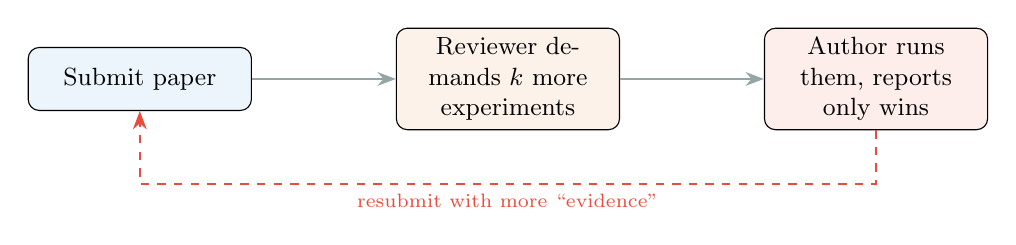
\begin{tikzpicture}[
  box/.style={draw,rounded corners,fill=#1!10,minimum width=2.8cm,minimum height=0.8cm,font=\small,align=center,text width=2.6cm},
  scale=0.85,
]
  \node[box=camera] (sub) at (0,0) {Submit paper};
  \node[box=counter] (rev) at (5.5,0) {Reviewer demands $k$ more experiments};
  \node[box=engine] (add) at (11,0) {Author runs them, reports only wins};

  \draw[-{Stealth},thick,neutral] (sub) -- (rev);
  \draw[-{Stealth},thick,neutral] (rev) -- (add);
  \draw[-{Stealth},thick,engine,dashed] (add.south) -- ++(0,-0.8) -| node[font=\scriptsize,below,pos=0.25] {resubmit with more ``evidence''} (sub.south);
\end{tikzpicture}
\end{center}

\vspace{0.5em}
{\small This is \textbf{counterperformativity}: the safety mechanism generates the risk it is designed to prevent. Same structure as the Gaussian copula in economics.}
\end{frame}

%% --- SLIDE: The data ---
\begin{frame}{The data: 11,196 ICLR submissions}

{\small We analyzed every public submission to \href{https://openreview.net/group?id=ICLR.cc/2024/Conference}{ICLR 2024} ($n = 7{,}404$) and \href{https://openreview.net/group?id=ICLR.cc/2023/Conference}{ICLR 2023} ($n = 3{,}792$).}

\vspace{0.5em}
{\small For each paper, we extracted:}
\begin{itemize}\setlength\itemsep{4pt}
  \item {\small Experiment demands from reviewer text}
  \item {\small Compliance signals from author rebuttals}
  \item {\small Final accept/reject decision}
\end{itemize}

\vspace{0.8em}
{\small \textbf{Headline:} papers that comply with experiment demands are accepted at \textbf{+10.7 pp} higher rates than those that don't.}

\vspace{0.5em}
{\small Sounds like the system works, right?}
\end{frame}

%% --- SLIDE: Data figure ---
\begin{frame}{Demand compliance and acceptance}
\begin{center}
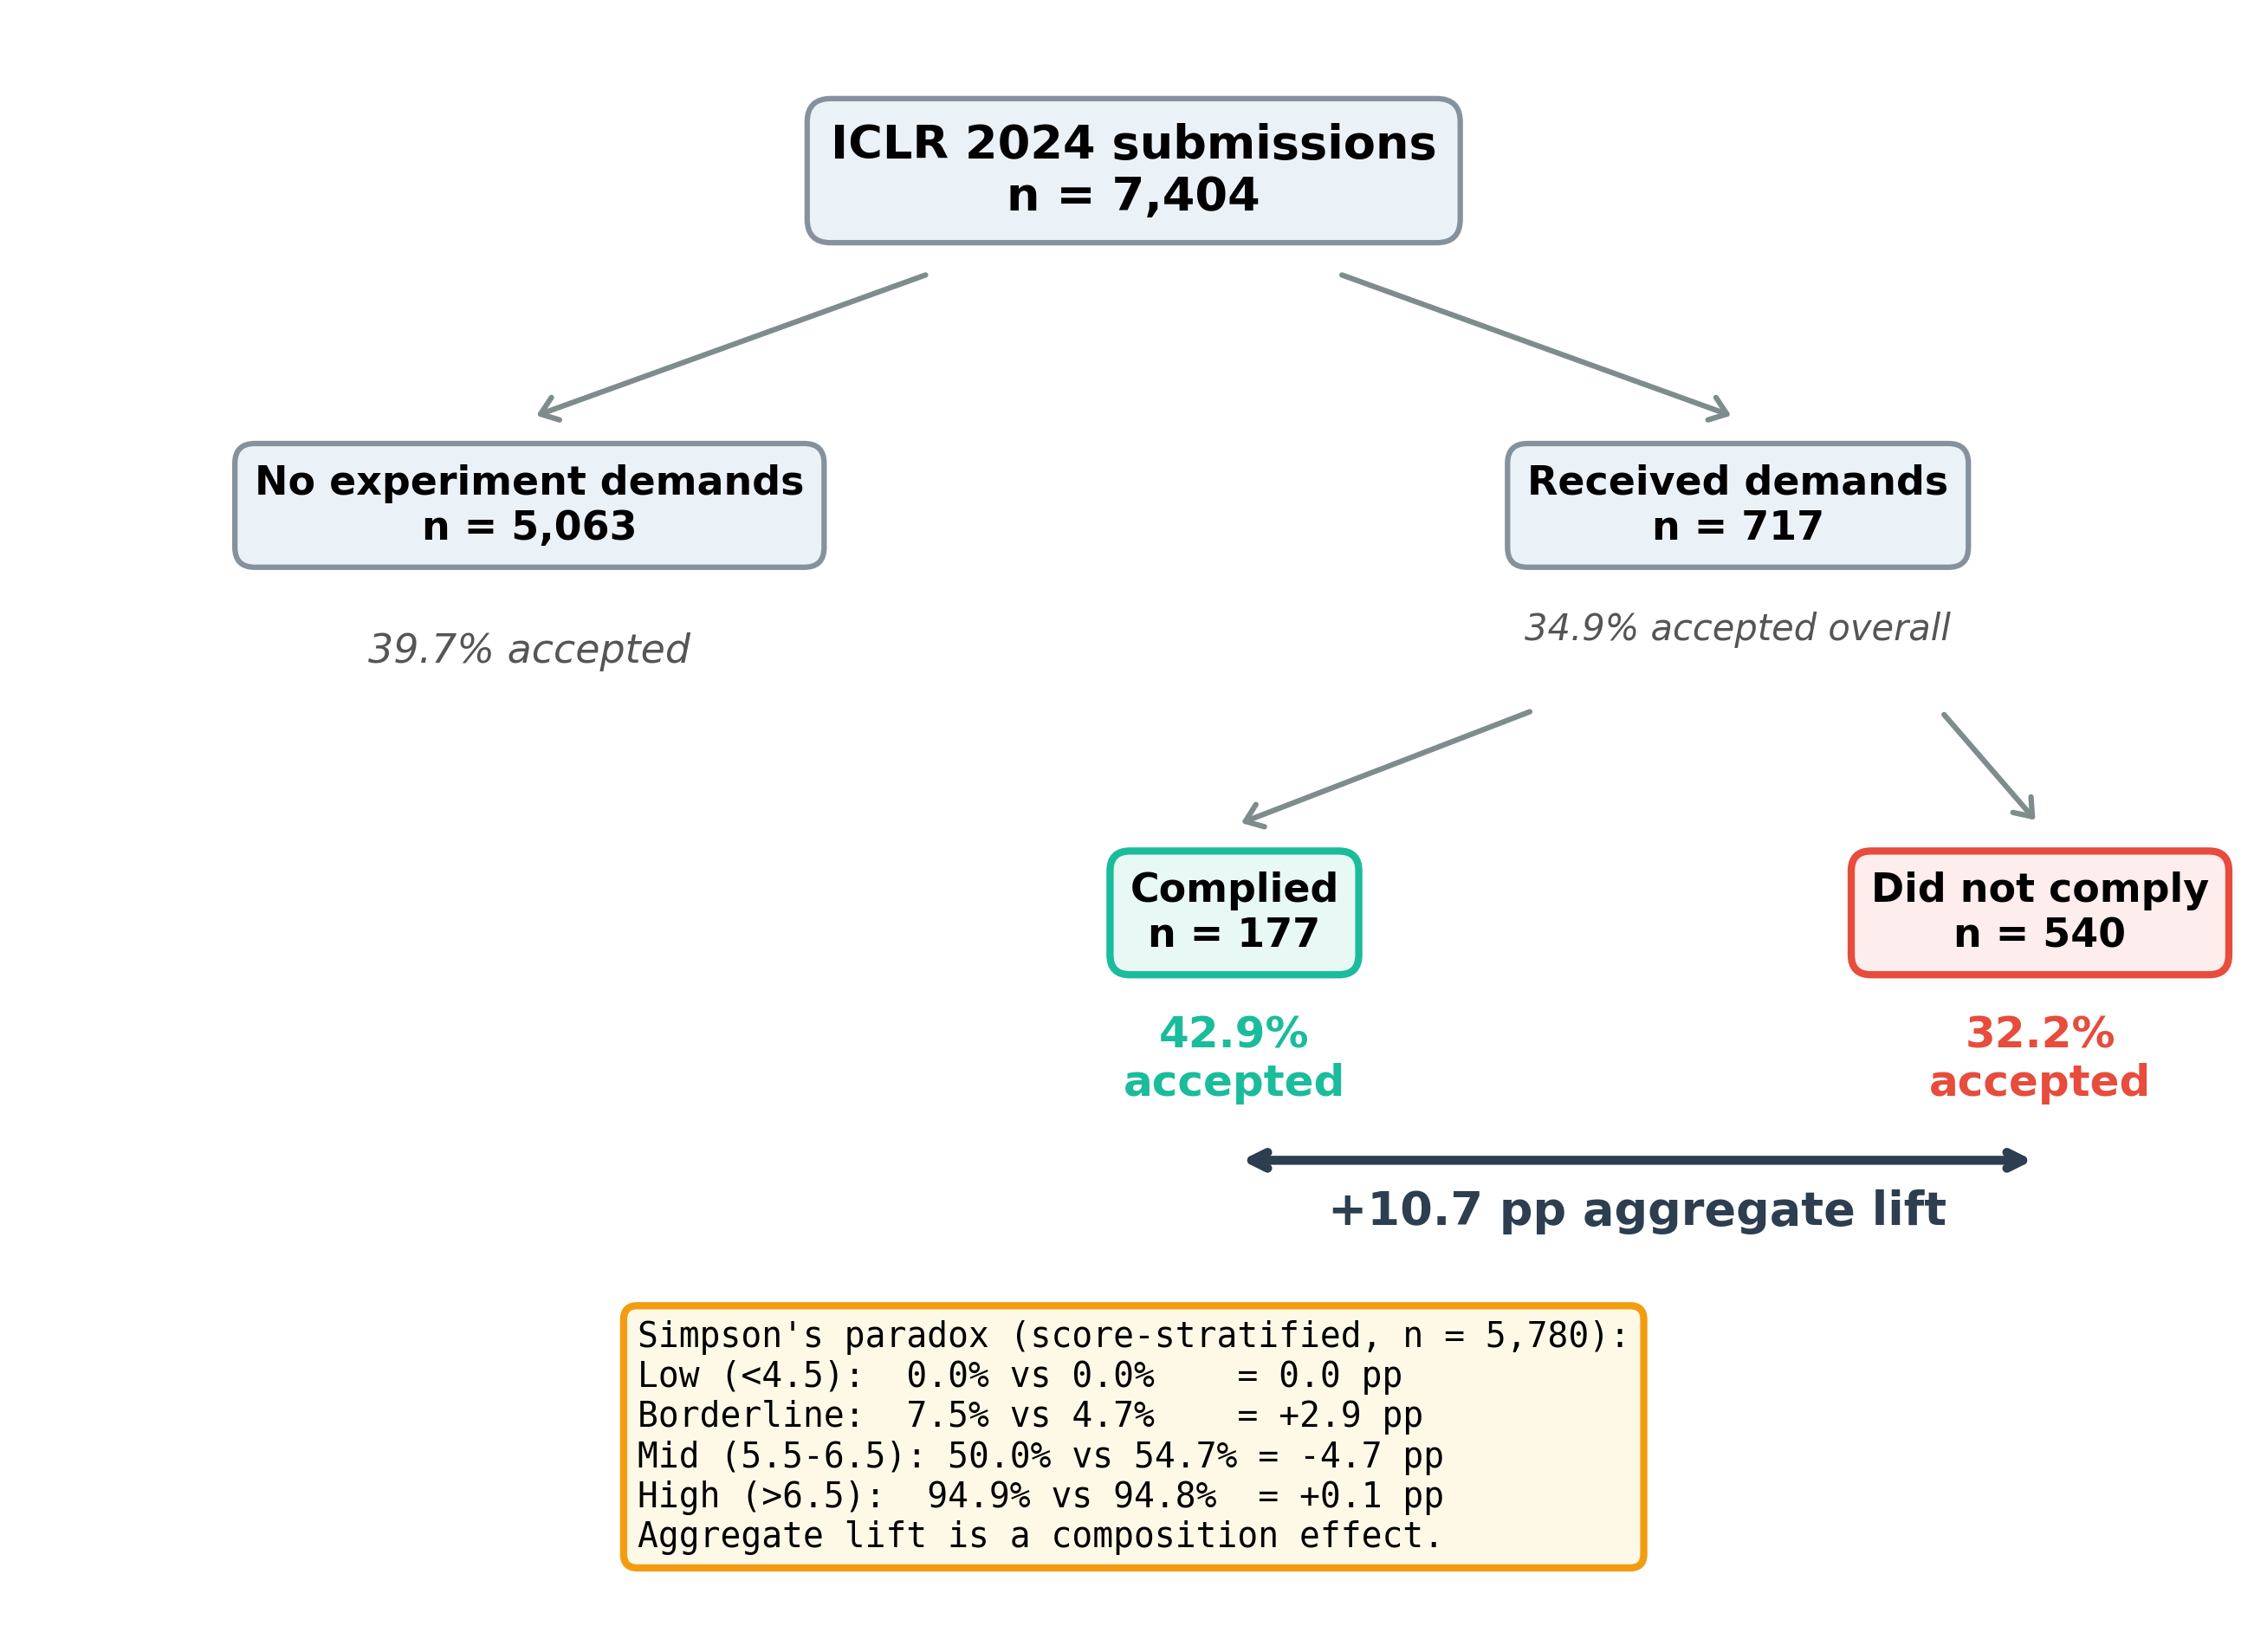
\includegraphics[width=0.8\linewidth]{fig7_demand_compliance.png}
\end{center}

\vspace{0.3em}
{\small Compliance with reviewer experiment demands correlates with acceptance --- but is the relationship causal, or a composition effect?}
\end{frame}

%% --- SLIDE: What is Simpson's paradox? ---
\begin{frame}{What is \href{https://en.wikipedia.org/wiki/Simpson\%27s_paradox}{Simpson's paradox}?}

A trend that appears in aggregate data \textbf{reverses} when you split the data into subgroups.

\vspace{0.5em}

\begin{columns}[T]
\begin{column}{0.48\textwidth}
\textbf{Classic example: Berkeley admissions}

\vspace{0.3em}
{\small In 1973, \href{https://en.wikipedia.org/wiki/Simpson\%27s_paradox\#UC_Berkeley_gender_bias}{UC Berkeley was sued for gender bias}: overall, men were admitted at higher rates than women.}

\vspace{0.3em}
{\small But when you looked \emph{department by department}, women were admitted at \textbf{equal or higher} rates in most departments.}

\vspace{0.3em}
{\small The aggregate gap existed because women applied to more competitive departments.}
\end{column}
\begin{column}{0.48\textwidth}
\textbf{The lesson}

\vspace{0.3em}
{\small An aggregate statistic can tell a completely different story from the stratified data.}

\vspace{0.5em}
{\small This matters whenever subgroups have different sizes \emph{and} different base rates.}

\vspace{0.5em}
{\small We found exactly this pattern in ICLR compliance data --- and it changes the interpretation entirely.}
\end{column}
\end{columns}
\end{frame}

%% --- SLIDE: Simpson's paradox in our data ---
\begin{frame}{Simpson's paradox: the lift is a composition effect}
\begin{columns}[T]
\begin{column}{0.55\textwidth}
{\small The +10.7 pp aggregate lift is a \textbf{Simpson's paradox}. When you stratify by reviewer score:}

\vspace{0.3em}

{\scriptsize
\begin{tabular}{lccr}
\toprule
\textbf{Stratum} & \textbf{Comply} & \textbf{No comply} & \textbf{Lift} \\
\midrule
Low ($<$4.5) & 0.0\% & 0.0\% & 0 pp \\
Border (4.5--5.5) & 7.5\% & 4.7\% & \textcolor{pass}{+2.9} pp \\
Mid (5.5--6.5) & 50.0\% & 54.7\% & \textcolor{fail}{$-$4.7} pp \\
High ($\geq$6.5) & 94.9\% & 94.8\% & +0.1 pp \\
\midrule
\textbf{Aggregate} & \textbf{42.9\%} & \textbf{32.2\%} & \textbf{+10.7} pp \\
\bottomrule
\end{tabular}
}

\vspace{0.3em}
{\small The lift \textbf{vanishes} within strata. The aggregate effect comes from composition: compliant papers cluster in the borderline stratum.}
\end{column}
\begin{column}{0.42\textwidth}
\vspace{0.5em}

{\small \textbf{Why this is worse, not better:}}

\vspace{0.3em}
{\small The compliance incentive concentrates \textbf{exactly where selective reporting is most consequential} --- borderline papers, where one more supportive experiment can tip the decision.}

\vspace{0.5em}
{\small For low-scored papers: compliance is \textbf{futile}.}

\vspace{0.2em}
{\small For high-scored papers: compliance is \textbf{unnecessary}.}

\vspace{0.2em}
{\small For borderline papers: compliance is \textbf{most tempting} and \textbf{least detectable}.}
\end{column}
\end{columns}
\end{frame}

%% --- SLIDE: Why this matters for performativity ---
\begin{frame}{Why this matters: performativity driven by a mirage}

{\small The aggregate data tells researchers: ``comply with experiment demands $\to$ get accepted.'' But the stratified data shows this is an illusion --- compliance doesn't actually help within any score band. So what's happening?}

\vspace{0.3em}

\begin{enumerate}\setlength\itemsep{3pt}
  \item {\small Researchers \emph{believe} more experiments $=$ acceptance (the aggregate signal)}
  \item {\small They optimize for compliance: run more benchmarks, add more ablations}
  \item {\small This doesn't actually improve their acceptance odds (the stratified signal)}
  \item {\small But it \emph{does} inflate the total number of implicit comparisons}
  \item {\small Which inflates the FWER --- more false positives enter the literature}
\end{enumerate}

\vspace{0.3em}

{\small The review system reshapes research behavior based on a statistical artifact. Researchers game a signal that isn't real --- and the gaming itself causes harm (more uncorrected comparisons). This is the counterperformative loop:}
\end{frame}

%% --- SLIDE: The loop diagram ---
\begin{frame}{The counterperformative loop}

\begin{center}
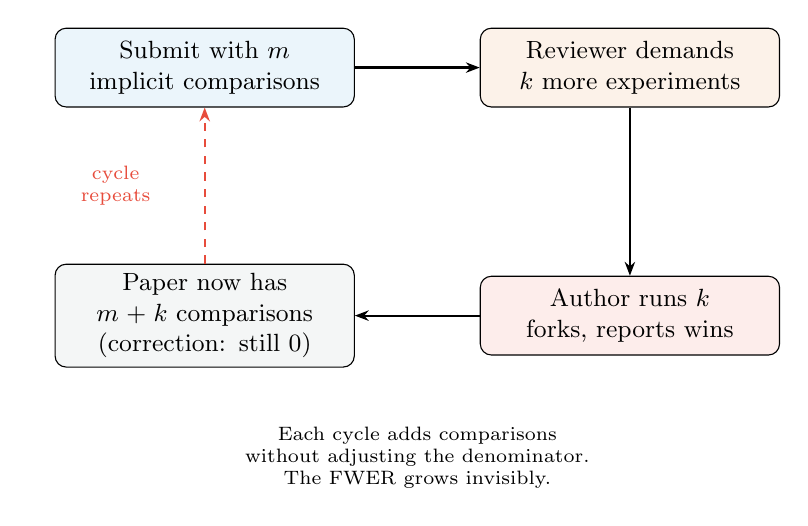
\begin{tikzpicture}[
  box/.style={draw,rounded corners,fill=#1!10,minimum width=3.8cm,minimum height=1cm,font=\small,align=center,text width=3.5cm},
  arr/.style={-{Stealth[length=5pt]},thick},
  scale=0.9,
]
  \node[box=camera] (sub) at (0,2) {Submit with $m$\\implicit comparisons};
  \node[box=counter] (rev) at (6,2) {Reviewer demands\\$k$ more experiments};
  \node[box=engine] (fork) at (6,-1.5) {Author runs $k$\\forks, reports wins};
  \node[box=neutral] (new) at (0,-1.5) {Paper now has\\$m + k$ comparisons\\(correction: still 0)};

  \draw[arr] (sub) -- (rev);
  \draw[arr] (rev) -- (fork);
  \draw[arr] (fork) -- (new);
  \draw[arr,engine,dashed] (new) -- node[font=\scriptsize,left,text width=2cm,align=center] {cycle\\repeats} (sub);

  % Annotation
  \node[font=\scriptsize,text width=4.5cm,align=center] at (3,-3.5) {Each cycle adds comparisons without adjusting the denominator.\\The FWER grows invisibly.};
\end{tikzpicture}
\end{center}
\end{frame}


%% ============================================================
%% PART 4: WHAT TO DO
%% ============================================================

\begin{frame}[plain]
\vfill
\begin{center}
  \setlength{\fboxrule}{2.5pt}%
  \fcolorbox{black}{white}{\parbox{0.55\textwidth}{\centering\vspace{0.8em}
    {\Large\bfseries Part 4}\\[0.5em]
    {\large What to do about it}
  \vspace{0.8em}}}
\end{center}
\vfill
\end{frame}

%% --- SLIDE: Interventions ---
\begin{frame}{Structural interventions}
\begin{columns}[T]
\begin{column}{0.48\textwidth}
\textbf{Make denominators visible}
\begin{itemize}\setlength\itemsep{1pt}
  \item {\small Report total experiments run, not just those in the paper}
  \item {\small For SAEs: report interpretability \emph{rates}, not cherry-picked features}
  \item {\small Template: ``trained $N$ features, $k$ scored above threshold $t$''}
\end{itemize}

\vspace{0.2em}
\textbf{Audit demands for FWER}
\begin{itemize}\setlength\itemsep{1pt}
  \item {\small Before demanding an ablation, ask whether it increases the comparison count}
  \item {\small Demand the correction alongside the experiment}
\end{itemize}
\end{column}
\begin{column}{0.48\textwidth}
\textbf{Publish negative results}
\begin{itemize}\setlength\itemsep{1pt}
  \item {\small \href{https://www.alignmentforum.org/posts/rPtLqBqiqrhswJfS8/research-we-didn-t-publish-2-mechanistic-interpretability}{GDM's ``research we didn't publish''} post is the template}
  \item {\small Venues should create tracks for replications and null results}
\end{itemize}

\vspace{0.2em}
\textbf{Bridge proof cultures}
\begin{itemize}\setlength\itemsep{1pt}
  \item {\small Cross-community benchmarks (\href{https://github.com/SAELens/SAEBench}{SAEBench}, \href{https://arxiv.org/abs/2410.15748}{MIB} are a start)}
  \item {\small Shared evaluation criteria across subfields}
  \item {\small Require engagement with alternative evidence standards in reviews}
\end{itemize}
\end{column}
\end{columns}
\end{frame}

%% --- SLIDE: Limitations ---
\begin{frame}{Project limitations}

\begin{enumerate}\setlength\itemsep{3pt}
  \item {\small \textbf{Observational.} The demand-compliance analysis is correlational. Simpson's paradox controls for quality, but within-stratum confounds remain.}

  \item {\small \textbf{One venue.} ICLR is the only major venue that publishes rejected submissions. Can't replicate at NeurIPS or ICML without the full corpus.}

  \item {\small \textbf{Effective, not Barnesian.} We claim benchmarks \emph{reshape} research priorities, not that the world conforms to the benchmark in the strong Black-Scholes sense.}

  \item {\small \textbf{No ethnography.} A proper sociology of MI would require interviews and lab observation, not just citation analysis.}

  \item {\small \textbf{Infrastructure gap.} Even if norms changed, experiment-tracking tools default to private. The tooling for public denominator reporting doesn't exist yet.}
\end{enumerate}
\end{frame}

%% --- SLIDE: Conclusion ---
\begin{frame}{Conclusion}

\begin{center}
\vspace{0.5em}
{\Large Statistical reform treats the \textbf{symptom}.}

\vspace{0.6em}

{\Large The cause is an evaluation culture whose}

\vspace{0.2em}

{\Large instruments both \textbf{\textcolor{camera}{measure}} and}

\vspace{0.2em}

{\Large \textbf{\textcolor{engine}{manufacture}} what counts as knowledge.}

\vspace{1.2em}

{\small The benchmark is an engine, not a camera.}

\vspace{0.2em}

{\small And like all engines, it needs maintenance, inspection,}

\vspace{0.1em}

{\small and occasionally --- replacement.}
\end{center}
\end{frame}

%% --- SLIDE: References/contact ---
\begin{frame}{Thank you}

\textbf{Paper:} TBD

\vspace{0.3em}
\textbf{Repository:} \href{https://github.com/elliottower/benchmarks-engines}{\texttt{github.com/elliottower/benchmarks-engines}}

\vspace{0.3em}
\textbf{Contact:} \texttt{elliot@elliottower.ai}

\vspace{0.5em}
\textbf{Key references:}
\begin{itemize}\setlength\itemsep{1pt}
  \item {\small MacKenzie (2006). \href{https://mitpress.mit.edu/9780262134606/an-engine-not-a-camera/}{\textit{An Engine, Not a Camera.}} MIT Press.}
  \item {\small MacKenzie (2001). \href{https://mitpress.mit.edu/9780262632959/mechanizing-proof/}{\textit{Mechanizing Proof.}} MIT Press.}
  \item {\small MacKenzie \& Bamford (2018). \href{https://doi.org/10.1080/13563467.2018.1505612}{Counterperformativity.} \textit{New Political Economy}.}
  \item {\small Espeland \& Sauder (2007). \href{https://doi.org/10.1086/517897}{Rankings and reactivity.} \textit{American Journal of Sociology}.}
\end{itemize}

\vspace{0.5em}
{\small Data: 11,196 ICLR submissions, 18 manual paper audits, OpenAlex citation analysis, Semantic Scholar citation network of 27 MI papers.}
\end{frame}

\end{document}
